
\documentclass{article}
\usepackage[spanish]{babel}
\usepackage[utf8]{inputenc}
\usepackage[backend=biber]{biblatex}
\bibliography{Referencias}
\usepackage[letterpaper,top=2.54cm,bottom=2.54cm,left=2.54cm,right=2.54cm,marginparwidth=1.75cm]{geometry}
\usepackage[rightcaption]{sidecap}
\usepackage{amsmath}
\usepackage{graphicx}
\usepackage[T1]{fontenc}
\usepackage{marvosym} 
\usepackage[document]{ragged2e}
\graphicspath{ {images} }
\usepackage{fancyhdr}
\usepackage{parskip}
\usepackage{fancyhdr}



\title{Tutorial de introducción a R}

\author{\text{Universidad Nacional De Colombia, Sede de La Paz}\\\\  Alvarez Martinez Jairo Alonso, Torres Bertel Luz Elenis \\ Gutierrez Navarro Ronald Andres}

\begin{document}
\maketitle
\thispagestyle{fancy}
\begin{Resumen}
\textbf{Resumen} \\\\
\justify{ En el presente documento se realizó un tutorial de información relevante del lenguaje de programación R, como lo son la instalación del mismo para un ordenador con sistema operativo windows y así mismo la instalación del entorno de RStudio con especificaciones sobre su interfaz. Se tuvieron en cuenta las personas que por algún motivo no deseen la instalación del programa en su computadora, por lo que se presentaron opciones varias para utilizar R online, se plantearon ejemplos a detalle sobre estructura de datos básica, como la creación de vectores, matrices y dataFrames, una vez detallado lo anterior mencionado, se ejemplifica un tipo de visualiación de datos, como lo es una gráfica de dispersión para su análisis, evidenciando la importancia de la visualización de datos cuando se requiere el análisis de datos.
}
\vspace{1em}\\
\textbf{Palabras Claves:}{programación, estadística,  computación, paradigma, digital
} \\
\end{Resumen}\\\\
\begin{Abstract}
\vspace{1em}
\textbf{Abstract} \\\\
\justify {In this document a tutorial of relevant information of the R programming language was made, such as the installation of the same for a computer with windows operating system and also the installation of the RStudio environment with specifications on its interface. We took into account people who for some reason do not want to install the program on their computer, so several options were presented to use R online, examples were given in detail on basic data structure, such as the creation of vectors, matrices and dataFrames, once detailed the above mentioned, a type of data visualization is exemplified, such as a scatter plot for analysis, demonstrating the importance of data visualization when data analysis is required.
}
\vspace{1em}\\
\textbf{Keywords:} {programming, statistics, computation, paradigm, digital} \\ \newpage
\end{Abstract}
\vspace{-6pt}\\

\justify{La realidad actual está convergiendo en torno a un paradigma digital, lo cual ha imprimido  un ritmo acelerado al dinamismo tecnológico impactado el mundo de forma positiva, en este enfoque la computación juega un papel relevante sirviendo como eje transversal a las diversas áreas de la investigación científica, el uso de un programa de computación en el campo de la Estadística es de gran importancia porque aumenta las posibilidades de automatización de los cálculos estadísticos para el análisis de los datos, lo que ha generado la necesidad de un lenguaje de programación orientado a satisfacer las necesidades en éste contexto (A. Martínez, S.Losa., 2017).

R es un lenguaje y entorno de programación para análisis estadístico que nos permite dar instrucciones, por medio de códigos, a nuestros equipos de cómputo para que realicen tareas  específicas, para saber algo del origen de R  es necesario aclarar  que se desprendió de S (statistical programing) dado que este programa era de uso restringido, Ross ihaka y Robert Gentleman crearon una versión libre y gratuita de S, lo cual terminó con la creación de R entre los años 1995 y 2000 (J. Mendoza.,2014). Cabe mencionar que Rstudio es un entorno de desarrollo integrado o IDE para la programación en R(H. Wickham, G. Grolemund, 2017).

Dentro de las características de la programación en  R resalta: la sencillez,la  eficacia, la inclusión de bucles, definición de funciones recursivas definidas por el usuario, facilidades en la entrada y salida, disposición de un eficaz sistema de manejo y almacenamiento de datos, ofrece un conjunto de operadores para realizar cálculos en matrices, listas, vectores y por último destacamos los equipamientos gráficos para el análisis y visualización de datos. En consecuencia a lo descrito anteriormente R es el lenguaje estadístico más utilizado a nivel mundial, logrando una aceptación generalizada en Universidades y en aplicaciones empresariales(Tutorials point, 2018).
}

\section{Instalación} 
\subsection{Instalación de R}
\justify {Pasos para la instalación local de R\\

"Para instalar R en tu computadora, ya sea de forma legal o gratuita, siga los pasos a continuación:
\\ Primero, dirijase al sitio web de R
y hacer lo siguiente (suponiendo que se trabaja en un
ordenador con sistema operativo Windows):
\begin{itemize}
    \item haga clic en descargar CRAN en la barra de la izquierda
    \item elija un sitio de descarga
    \item elija Windows como sistema operativo de destino
    \item haga clic en la base
    \item elija Descargar R 4.2.0 para Windows † y elija las respuestas por defecto para todas las preguntas También es posible ejecutar R y RStudio desde una memoria USB en lugar de instalarlos, Este puede ser útil cuando no se tienen derechos de administradores en su ordenador
\end{itemize}
\newpage
\subsection{Instalar RStudio}
\justify{
Después de terminar esta instalación, debería ver un icono de R en tu escritorio. Al hacer clic en él, se iniciará
la interfaz estándar. Sin embargo, le recomendamos que utilice la interfaz de RStudio.\\
Para Instalar Rstudio, siga los pasos a continuación:
\begin{itemize}
    \item dirijase a http://www.rstudio.org/ y haga lo siguiente (suponiendo que trabaja en una computadora con sistema operativo windows):
    \item haga clic en Descargar RStudio
    \item haga clic en Descargar RStudio Desktop
    \item haga clic en Recomendado para su sistema
    \item descargue el archivo .exe y ejecútelo (elija las respuestas por defecto para todas las preguntas)
\end{itemize}
}
\subsection{Diseño de RStudio}
\justify{
La interfaz de RStudio consta de varias ventanas
\begin{center}
    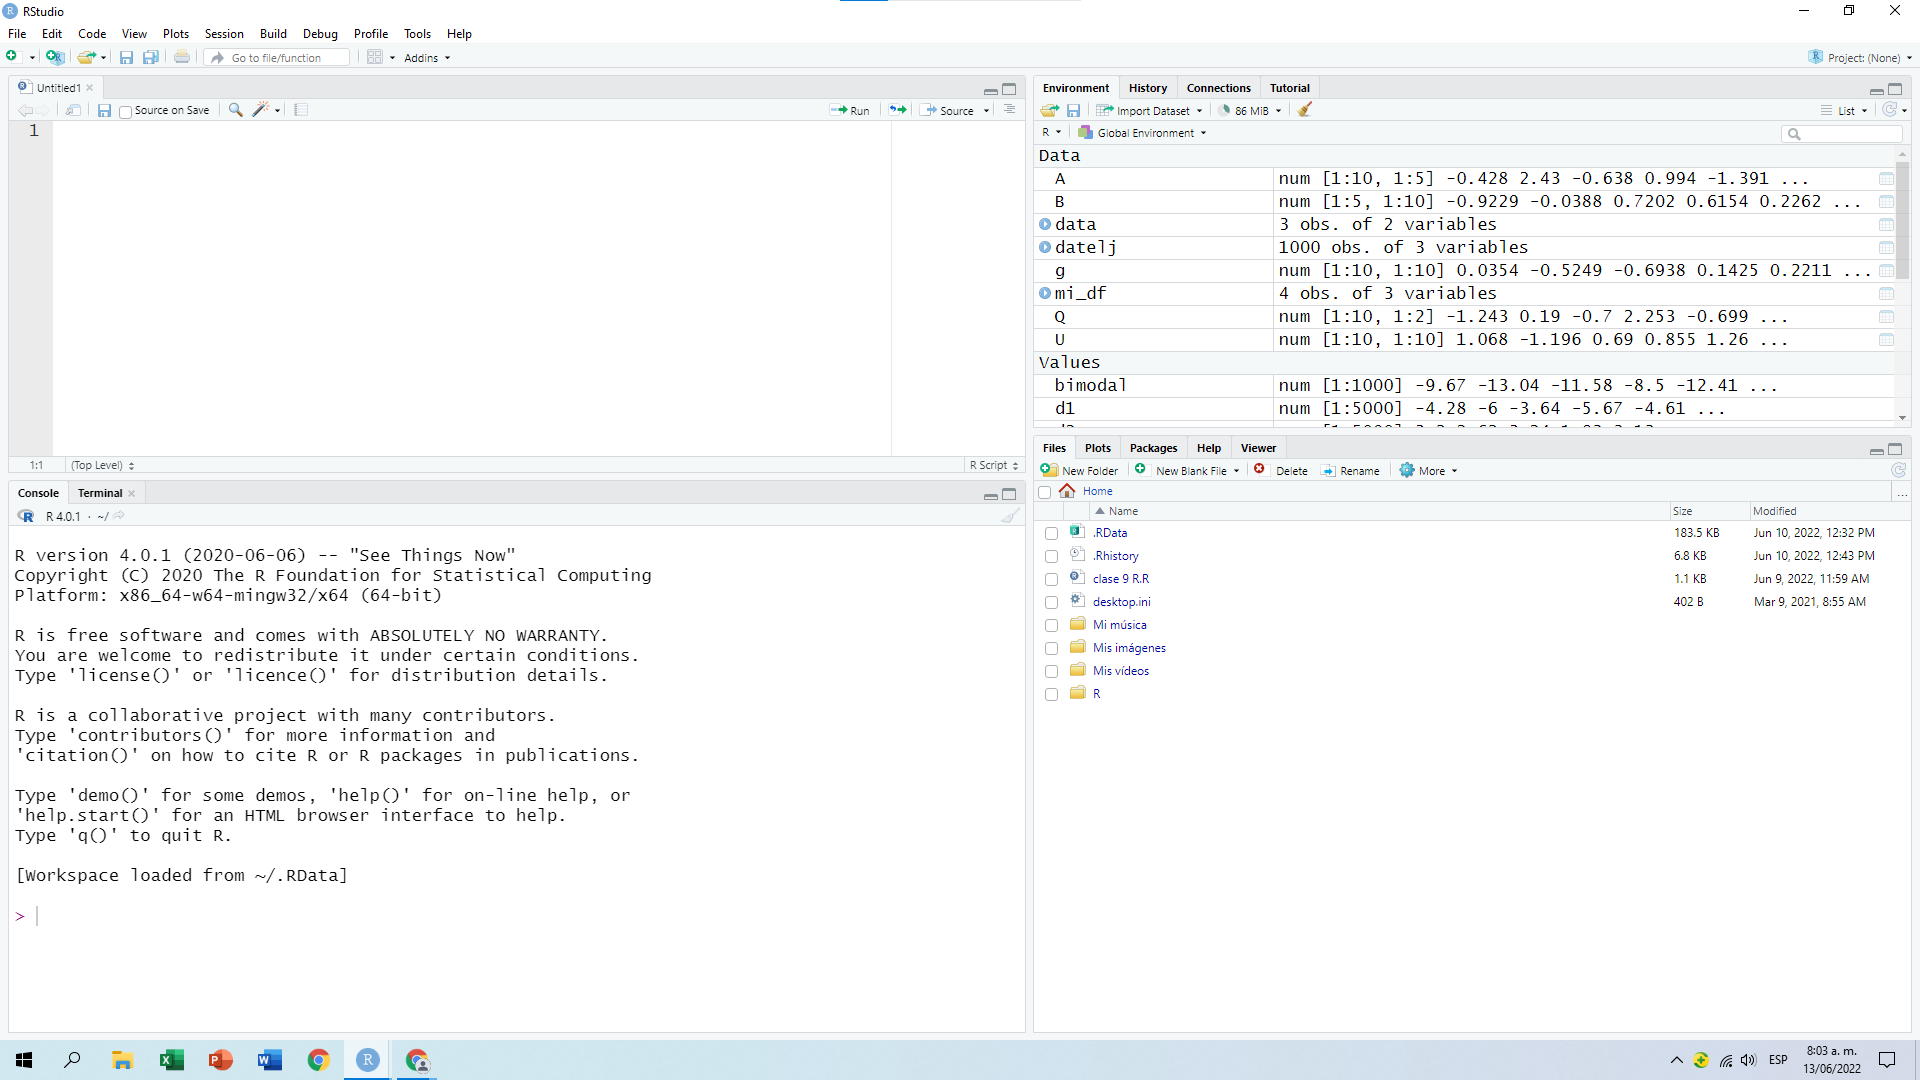
\includegraphics[width=10cm, height=6cm]{Rstudio.png}\\
    \caption{Interfaz de Rstudio}
\end{center}
}
\begin{itemize}
    \item Abajo a la izquierda: ventana de la consola (también llamada ventana de comandos). Aquí puede escribir comandos simples después de la indicación ">" y R ejecutará su comando. Esta es la ventana más importante, porque aquí es donde R realmente hace cosas.
    \item Arriba a la izquierda: ventana del editor (también llamada ventana de Colecciones de comandos scripts) aquí pueden ser editados y guardados los comandos.
    \item Arriba a la derecha: espacio de trabajo / ventana del historial. En la ventana del espacio de trabajo puede ver qué datos y valores que R tiene en su memoria. Usted Puede ver y editar los valores haciendo clic en en ellos. La ventana del historial muestra lo que se ha sido tecleado antes.
    \item Abajo a la derecha: archivos / gráficos / paquetes / ventana de ayuda. Aquí puede abrir archivos, ver los gráficos (también los anteriores), instalar y cargar paquetes o utilizar la función de ayuda
\end{itemize}

Nota: Puede cambiar el tamaño de las ventanas arrastrando las barras grises entre las ventanas.
arrastrando las barras grises entre las ventanas."  (Torfs, P. J. J. F., & Brauer, C. C, 2012)
}
\newpage
\section{Alternativas de ejecución de R en la web}
En la web existen múltiples entornos de desarrollo en R, por lo que a continuación se mostrarán tres de ellos, en los que se recomienda trabajar por su uso poco complejo:
\justify{
\begin{itemize}
    \item https://rdrr.io/snippets/
    \item https://paiza.io/es/projects/new?language=r
    \item https://rstudio.cloud/
\end{itemize}

}

\section{Estructuras de datos básicas}
\justify{ 
\begin{itemize}
    \item Vectores
    \item Matrices
    \item Data frames
\end{itemize}
}

\subsection{Vectores}
Los vectores son una colección de datos del mismo tipo concatenados con la función c(). Esto último es muy importante ternelo en cuenta, puesto que si distintos tipos de datos se agrupan en un vector, ocurre lo que se conoce como coerción de tipos de datos, es decir, los componentes se transfroman en elementos del mismo tipo   \\coercion <- c(TRUE, "\ Correct\ ", 8, 2.2)\\
class(coercion)\\
typeof(coercion)\\
\\Si ejecutamos el código anterior, el resulado será:\\
\\TRUE, Correct, 8, 2.2\\
character\\
character\\
\\Observamos que, aunque en teoría el vetor «coercion» contiene distintos tipos de datos, se aplica la coerción de tipos de datos y todos los elemntos terminan siendo del mismo tipo, como lo muestran las funciones class() y typeof(). (Vectores en R, R CODER) \\

\subsection{Matrices}
\justify{Las matrices, al igual que los vectores, son  arreglos o conjuntos que contienen el mismo tipo de dato. Sin embargo, a diferencia de los vectores, una matriz puede poseer tanto filas como columnas.\\
\\Por ejemplo, la siguiente matriz en R consta de una columna y seis filas:\\
\\data <- 1:6\\
matrix(data)\\
}
Si ejecutamos el comando anterior, obtenemos como resultado:\\
\begin{center}

    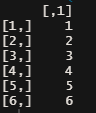
\includegraphics[width=3cm,height=4cm]{matriz.png}\\
    \caption{Figura 1: Matriz de 6x1}
    
\end{center} 
\subsection{Dataframe}
\justify{
A diferencia de los vectores y las marices, los "Data Frames" (marcos de datos), pueden contener diferentes tipos de datos. Un ejemplo de un data frame en R es el siguiente:} \\

\begin{center}
       
    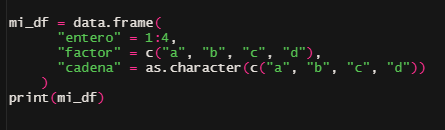
\includegraphics[width=9cm, height=3cm]{dataF.png}\\
    \caption{Figura 2:código de dataFrame}
    
\end{center}

\\Si ejecutumos las líenas del código anterior, obtenemos como resultado:\\ 

\begin{center}
    

    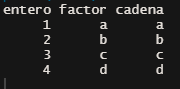
\includegraphics[width=5cm, height=3cm]{dta.png}\\
    \caotion{Figura 3: dataFrame}
    
\end{center}

\section{Opciones y ejemplos de visualización de datos.}
\justify{ R presenta gran variedad de opciones para graficar datos obtenidos de información externa o registrada directamente en el programa, como lo son los gráficos de "tallos y hojas", de "puntos" (dot plots), gráficos de barras (bar charts), histogramas, gráficos de densidad kernel, diagrama de cajas (box plots), diagramas de violín y gráficos de dispersión. En esta ocación trabajaremos con comandos básicos. A continuación se describirán los pasos para la visualización de datos obtenidos de un archivo de excel.
\begin{enumerate}
    \item Cargamos el paquete readx1()
    \item Buscamos la ruta del archivo de excel
    \item Copiamos la ruta de la consola y la guardamos en una variable
    \item Miramos  las hojas del excel en donde están ubicados los datos
    \item Guardamos los datos en una variable
    \item Con el comando plot, imprimimos los datos en una gráfica de dispersión
\end{enumerate}

\begin{center}
    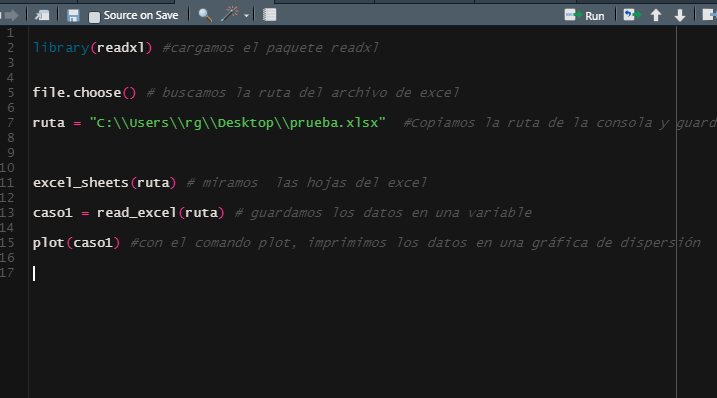
\includegraphics[width=10cm, height=6cm]{code.png}\\
\end{center}

Si ejecutamos las líneas de código anterior, obtenemos los siguientes resultados:

\begin{center}
    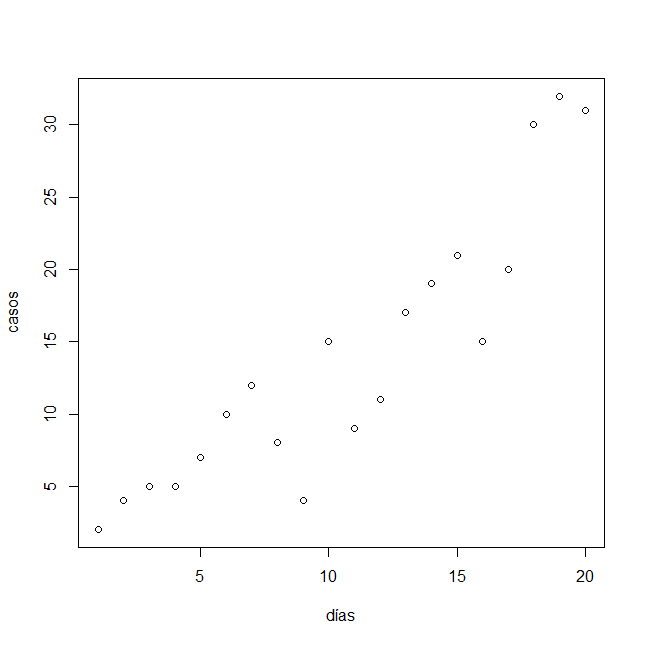
\includegraphics[width=10cm, height=7cm]{grafica.png}\\
\end{center}
Si desea jugar con la consola y graficar las otras opciones anteriormente descritas puedes visitar \\ https://xwiki.recursos.uoc.edu/wiki/mat71575es/view/Main/Visualizaci\%C3\%B3n\%20de\%20datos\%20en\%20R, un sitio web que cuenta con una guía que te indicará paso a paso cómo ilustrar los datos que requieras
}

\newpage

\begin{thebibliography}{20}

\bibitem{refarticle1}
Vectores en R. (s. f.). R CODER. https://r-coder.com/vectores-r/

\bibitem{refarticle2}
Torfs, P. J. J. F., & Brauer, C. C. (2012). A (very) short introduction to R. Wageningen UR. http://cran.r-project.org/doc/contrib/Torfs+Brauer-Short-R-Intro.pdf

\bibitem{refarticle3}
Avello Martínez, R., & Seisdedo Losa, A. (2017). El procesamiento estadístico con R en la investigación científica. MediSur, 15(5), 583-586.

\bibitem{refarticle4}
Copyright © 2017 Garrett Grolemund, Hadley Wickham. All rights reserved. Printed in Canada.

\bibitem{refarticle5}
Copyright 2018 by Tutorials Point (I) Pvt. Ltd.

\end{thebibliography}



\end{document}
